\chapter{Anexo A}
\label{cap:AnexoA}

Este anexo se ha dedicado a los diagramas de secuencia de los casos de uso más interesantes.

\begin{itemize}
	\item\textbf{Iniciar sesión}, en la figura \ref{Fig:dia_iniciarsesion}. También se muestra aquí, de manera opcional, cómo se podría cambiar la apariencia visual del programa.
	\item\textbf{Visualizar las notas del alumno}, en la figura \ref{Fig:dia_mainwindow} para las notas finales y en la figura \ref{Fig:dia_informealumno} para el informe general del alumno.
	\item\textbf{Crear una nueva prueba}, en la figura \ref{Fig:dia_nuevaprueba}.
	\item\textbf{Calificar una prueba}, en la figura \ref{Fig:dia_calificarprueba}.
	\item\textbf{Modificar una prueba}, en la figura \ref{Fig:dia_modificarprueba}.
	\item\textbf{Borrar una prueba}, en la figura \ref{Fig:dia_borrarprueba}.
	\item\textbf{Editar datos del usuario}, en la figura \ref{Fig:dia_editarusuario}.
	\item\textbf{Cargar alumnos}, en las figuras \ref{Fig:dia_cargaralumno} para un solo alumno y \ref{Fig:dia_cargaralumnos} para varios alumnos.
\end{itemize}

\begin{figure}[h]
\centering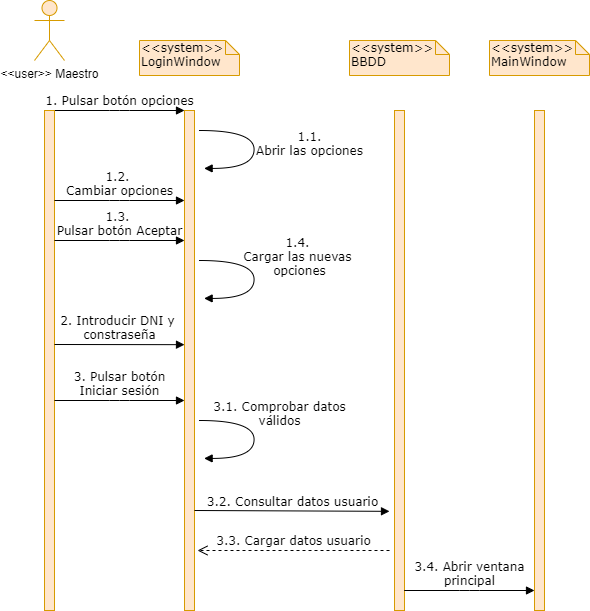
\includegraphics[width=1\linewidth]{figs/dia_iniciarsesion.png}
\caption{Diagrama de secuencia del inicio de sesión.}
\label{Fig:dia_iniciarsesion}
\end{figure}

\begin{figure}[h]
\centering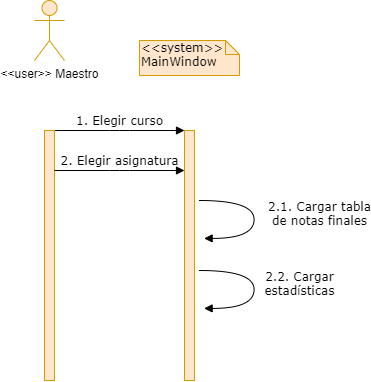
\includegraphics[width=1\linewidth]{figs/dia_mainwindow.png}
\caption{Diagrama de secuencia de la visualización de notas finales.}
\label{Fig:dia_mainwindow}
\end{figure}

\begin{figure}[h]
\centering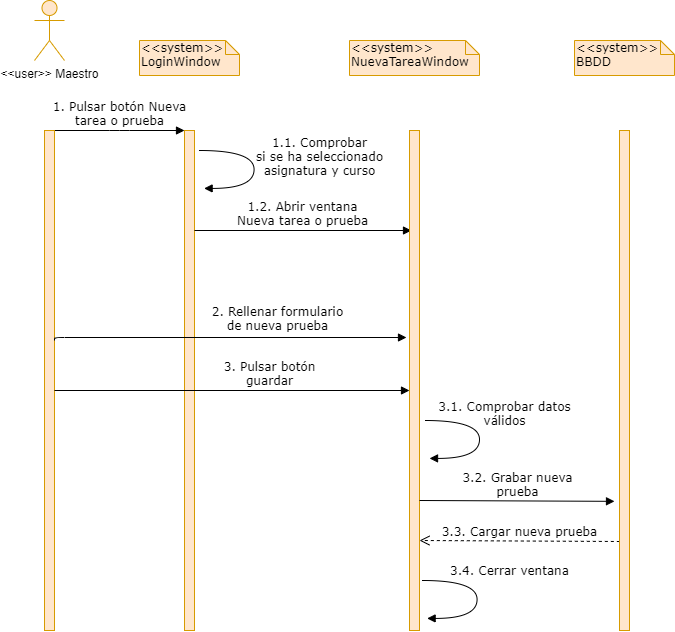
\includegraphics[width=1\linewidth]{figs/dia_nuevaprueba.png}
\caption{Diagrama de secuencia de la creación de una prueba nueva.}
\label{Fig:dia_nuevaprueba}
\end{figure}

\begin{figure}[h]
\centering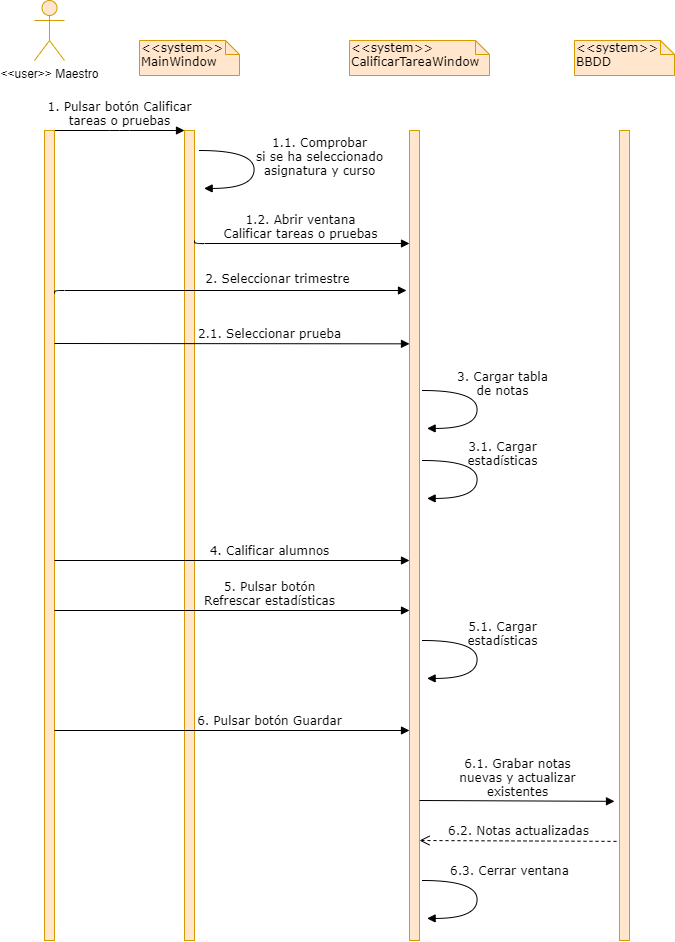
\includegraphics[width=1\linewidth]{figs/dia_calificarprueba.png}
\caption{Diagrama de secuencia de la calificación de una prueba.}
\label{Fig:dia_calificarprueba}
\end{figure}

\begin{figure}[h]
\centering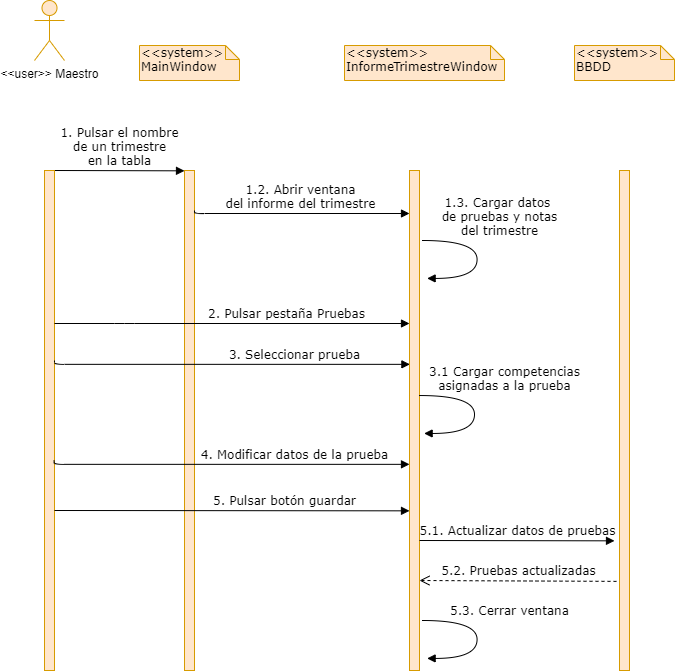
\includegraphics[width=1\linewidth]{figs/dia_modificarprueba.png}
\caption{Diagrama de secuencia de la modificación de una prueba.}
\label{Fig:dia_modificarprueba}
\end{figure}

\begin{figure}[h]
\centering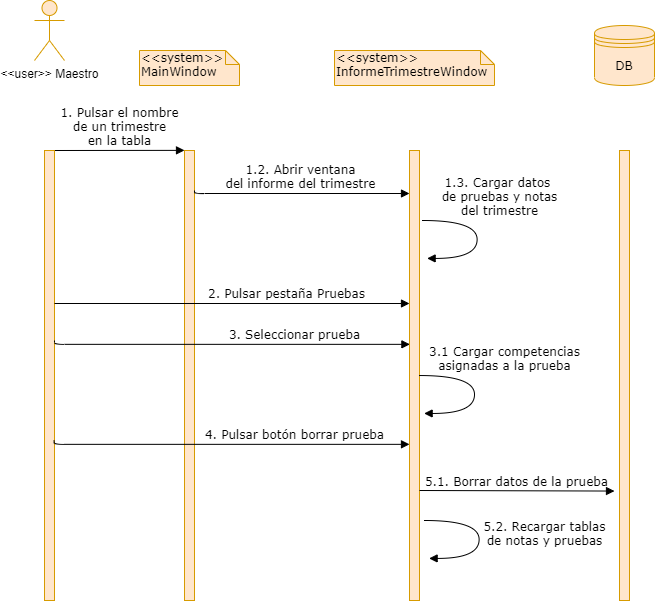
\includegraphics[width=1\linewidth]{figs/dia_borrarprueba.png}
\caption{Diagrama de secuencia del borrado de una prueba.}
\label{Fig:dia_borrarprueba}
\end{figure}

\begin{figure}[h]
\centering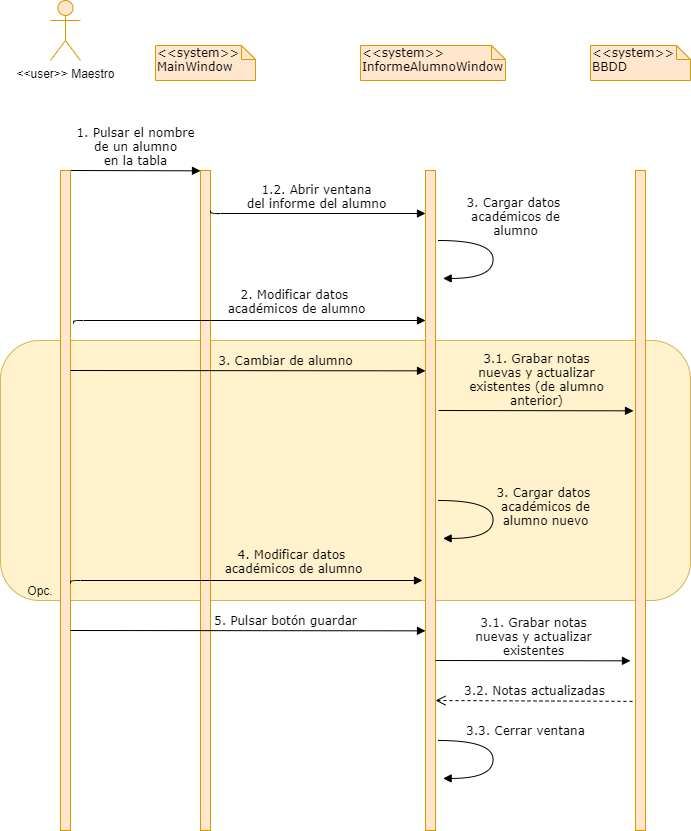
\includegraphics[width=1\linewidth]{figs/dia_informealumno.png}
\caption{Diagrama de secuencia de la visualización de todas las notas del alumno.}
\label{Fig:dia_informealumno}
\end{figure}

\begin{figure}[h]
\centering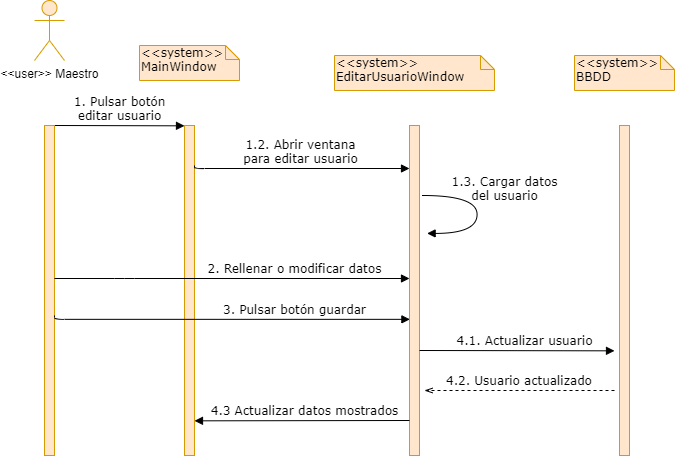
\includegraphics[width=1\linewidth]{figs/dia_editarusuario.png}
\caption{Diagrama de secuencia de la edición de los datos del usuario.}
\label{Fig:dia_editarusuario}
\end{figure}

\begin{figure}[h]
\centering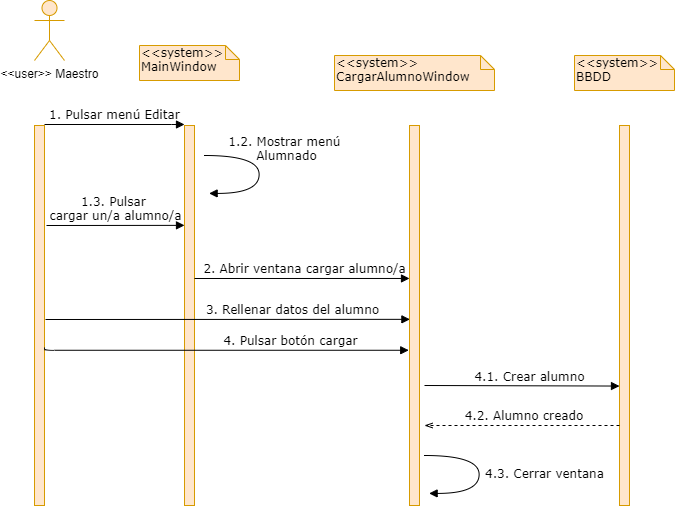
\includegraphics[width=1\linewidth]{figs/dia_cargaralumno.png}
\caption{Diagrama de secuencia de la carga de un alumno.}
\label{Fig:dia_cargaralumno}
\end{figure}

\begin{figure}[h]
\centering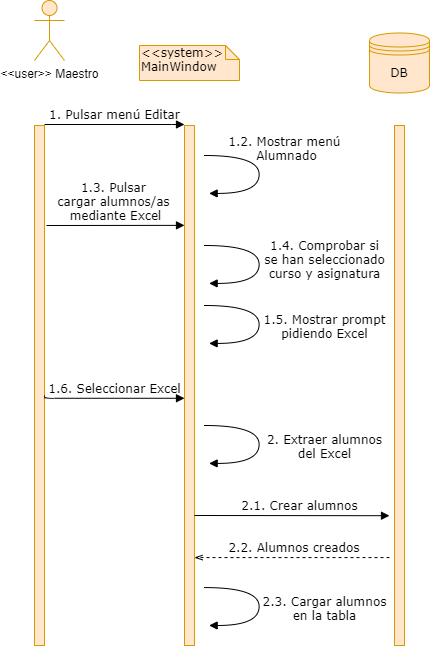
\includegraphics[width=0.5\linewidth]{figs/dia_cargaralumnos.png}
\caption{Diagrama de secuencia de la carga de varios alumnos.}
\label{Fig:dia_cargaralumnos}
\end{figure}